%%%%%%%%%%%%%%%%%%%%%%%%%%%%%%%%%%%%%%%%%%%%%%%%%%%%%%%%%%%%%%%%%%%%%%%%
% UNIBOARD LATEX TEMPLATE
%%%%%%%%%%%%%%%%%%%%%%%%%%%%%%%%%%%%%%%%%%%%%%%%%%%%%%%%%%%%%%%%%%%%%%%%

\documentclass[oneside]{scrreprt}


\usepackage{import}
\import{latex/}{english.tex} 
\usepackage{listings}
\usepackage{cleveref}
% you must set the path according to the current document folder
% use "german.tex" for documents in german and "english.tex" for
% documents in english
\inputpath{{listings/}{figures/}}
%\usepackage{bera}% optional: just to have a nice mono-spaced font
\usepackage{listings}
\usepackage{xcolor}

\colorlet{punct}{red!60!black}
\definecolor{background}{HTML}{EEEEEE}
\definecolor{delim}{RGB}{20,105,176}
\colorlet{numb}{magenta!60!black}

\lstdefinelanguage{json}{
    basicstyle=\normalfont\ttfamily,
    numbers=left,
    numberstyle=\scriptsize,
    stepnumber=1,
    numbersep=8pt,
    showstringspaces=false,
    breaklines=true,
    frame=lines,
    backgroundcolor=\color{background},
    literate=
     *{0}{{{\color{numb}0}}}{1}
      {1}{{{\color{numb}1}}}{1}
      {2}{{{\color{numb}2}}}{1}
      {3}{{{\color{numb}3}}}{1}
      {4}{{{\color{numb}4}}}{1}
      {5}{{{\color{numb}5}}}{1}
      {6}{{{\color{numb}6}}}{1}
      {7}{{{\color{numb}7}}}{1}
      {8}{{{\color{numb}8}}}{1}
      {9}{{{\color{numb}9}}}{1}
      {:}{{{\color{punct}{:}}}}{1}
      {,}{{{\color{punct}{,}}}}{1}
      {\{}{{{\color{delim}{\{}}}}{1}
      {\}}{{{\color{delim}{\}}}}}{1}
      {[}{{{\color{delim}{[}}}}{1}
      {]}{{{\color{delim}{]}}}}{1},
}

% Systems
\newcommand{\univote}{\mbox{UniVote}}
\newcommand{\uniboard}{\mbox{UniBoard}}
\newcommand{\unicert}{\mbox{UniCert}}
\newcommand{\fig}[1]{Figure~ref{#1}}

\begin{document}

\lstset{
  language=Java,
  basicstyle=\footnotesize\sffamily, %\sffamily, \ttfamily
  keywordstyle=\bfseries,
  numbers=right
}

\title{UniCert Architecture Specification}
\maketitle

\begin{versionhistory}
	\vhEntry{0.1}{September 10, 2014}{Philémon von Bergen}{Initial draft.}
\end{versionhistory}

%%%%%%%%%%%%%%%%%%%%%%%%%%%%%%%%%%%%%%%%%%%%%%%%%%%%%%%%%%%%%%%%%%%%%%%%
%\chapter*{Abstract}
%%%%%%%%%%%%%%%%%%%%%%%%%%%%%%%%%%%%%%%%%%%%%%%%%%%%%%%%%%%%%%%%%%%%%%%%


%%%%%%%%%%%%%%%%%%%%%%%%%%%%%%%%%%%%%%%%%%%%%%%%%%%%%%%%%%%%%%%%%%%%%%%%

\tableofcontents

%%%%%%%%%%%%%%%%%%%%%%%%%%%%%%%%%%%%%%%%%%%%%%%%%%%%%%%%%%%%%%%%%%%%%%%%
\chapter{Introduction}
%%%%%%%%%%%%%%%%%%%%%%%%%%%%%%%%%%%%%%%%%%%%%%%%%%%%%%%%%%%%%%%%%%%%%%%%

This document presents the architectural specification of \unicert. \unicert\ is a certification authority, that issues digital certificates used to authenticate users, to sign and/or encrypt messages. \unicert\ provides an interface where the user can authenticate themselves and request predefined parameters that must appear in the certificate they will ask \unicert\ to issue. \unicert\ uses \uniboard\ to publish all issued certificates. A general description of what \unicert\ does and how it works is available in document \cite{univote_spec}. 

This document presents the detailed certificate issuing process and focuses on architectural and technical specifications. In a \Cref{chap:process}, the components and processes of authentication and issuance of the certificate will be described in more details. \Cref{chap:architecture} describes the architecture of some important classes. Finally, \Cref{chap:specialities} describes some important \unicert\ particularities.

%%%%%%%%%%%%%%%%%%%%%%%%%%%%%%%%%%%%%%%%%%%%%%%%%%%%%%%%%%%%%%%%%%%%%%%%
\chapter{Components and Processes} \label{chap:process}
%%%%%%%%%%%%%%%%%%%%%%%%%%%%%%%%%%%%%%%%%%%%%%%%%%%%%%%%%%%%%%%%%%%%%%%%

To give an overview of how \unicert\ works, we give a high-level picture of the architecture and the processes that compose \unicert.

\section{Components}

\unicert\ is composed of two components. The fist one, the authentication component called \textit{unicert-authentication}, has following functions:
\begin{itemize}
\item authenticate the user
\item allow the user to get predefined parameters that must appear in a certificate
\item send all data to issuer component
\item return the private key (generated on user side) and the issued certificate (received from the issuer component) to the user.
\end{itemize}
The application using \unicert\ is responsible for generating the key pair and choosing other values to certify. \unicert\ provides only a test user interface for these tasks.

The second component, the issuer component called \textit{unicert-issuer}, has following functions:
\begin{itemize}
\item issue the certificate based on the data received
\item post the certificate on \uniboard
\item return the certificate to the authentication component
\end{itemize}

\section{Authentication Process} \label{sec:auth_process}


Currently, the authentication component supports two identity providers to authenticate the user, namely SwitchAAI and Google. Even they do not use the same technologies, the flow of the authentication process is similar. Their concrete implementation differ however slightly. The authentication process shows in \Cref{fig:auth_process} is described below.

To begin the procedure, the user asks the application using \unicert\ to authenticate themselves. The application calls the \textit{AuthenticationServlet} of \textit{unicert-authentication} providing the identifier of a parameter set and the return url that will by called by \textit{unicert-authentication} at the end of the authentication process to go back to the application. \textit{AuthenticationServlet} reads the parameter set provided (purpose of this set will be described in \Cref{sec:param_request}) and saves it in the session together with the return url. If multiple identity providers are defined in the parameter set, \textit{unicert-authentication} shows the \textit{idpselection.xhtml} page where the user can choose the desired identity providers. \textit{AuthenticationServlet} then makes a redirect on identity provider authentication page where the user can process to the login. If the login process is successful, the identity provider returns user attributes to \textit{SwitchAAICallbackServlet} (in case of SwitchAAI) or \textit{OAuth2CallbackServlet} (in case of Google). Theses servlets save the user attributes in the session and call the \textit{CallbackServlet}. This servlet call the 
return url passing the session id back to the application.

At the end of the authentication process, the application has an authenticated session on \textit{unicert-authentication} for this user.

%\paragraph*{SwitchAAI authentication} SwitchAAI uses a Shibboleth module of Apache webserver to make the redirection to the authentication webpage and back. \Cref{fig:auth_process_switch} shows how the process works. To begin the procedure, the user must invoke a link containing some information about what parameters must be loaded for the authentication and issuance process (described in more details later in \Cref{sec:simplification_ui}). This can for example be done by clicking on a link on the home page of \unicert. This link calls the \textit{ParameterServlet} which loads the required parameters, among others the supported identity providers for authentication. If more than one are supported, page \textit{idpselection.xhtml} is displayed where the user can choose which provider to use.

%For the present case, SwitchAAI is selected. Page \textit{switchaai.xhtml} is requested. For this page, the Apache Shibboleth module expects a valid user to be logged in. If it is not the case, the user is redirected to SwitchAAI authentication page. Once the credentials entered and the user successfully authenticated by SwitchAAI, the Apache Shibboleth module verifies the response received from Switch and displays the \textit{switchaai.xhtml} page where the user personal information received from Switch are read. After a few seconds, the user is redirected to the page where the certificate can be requested (\textit{certificate-request.xhtml}).

\begin{figure}[ht]
\centerline{
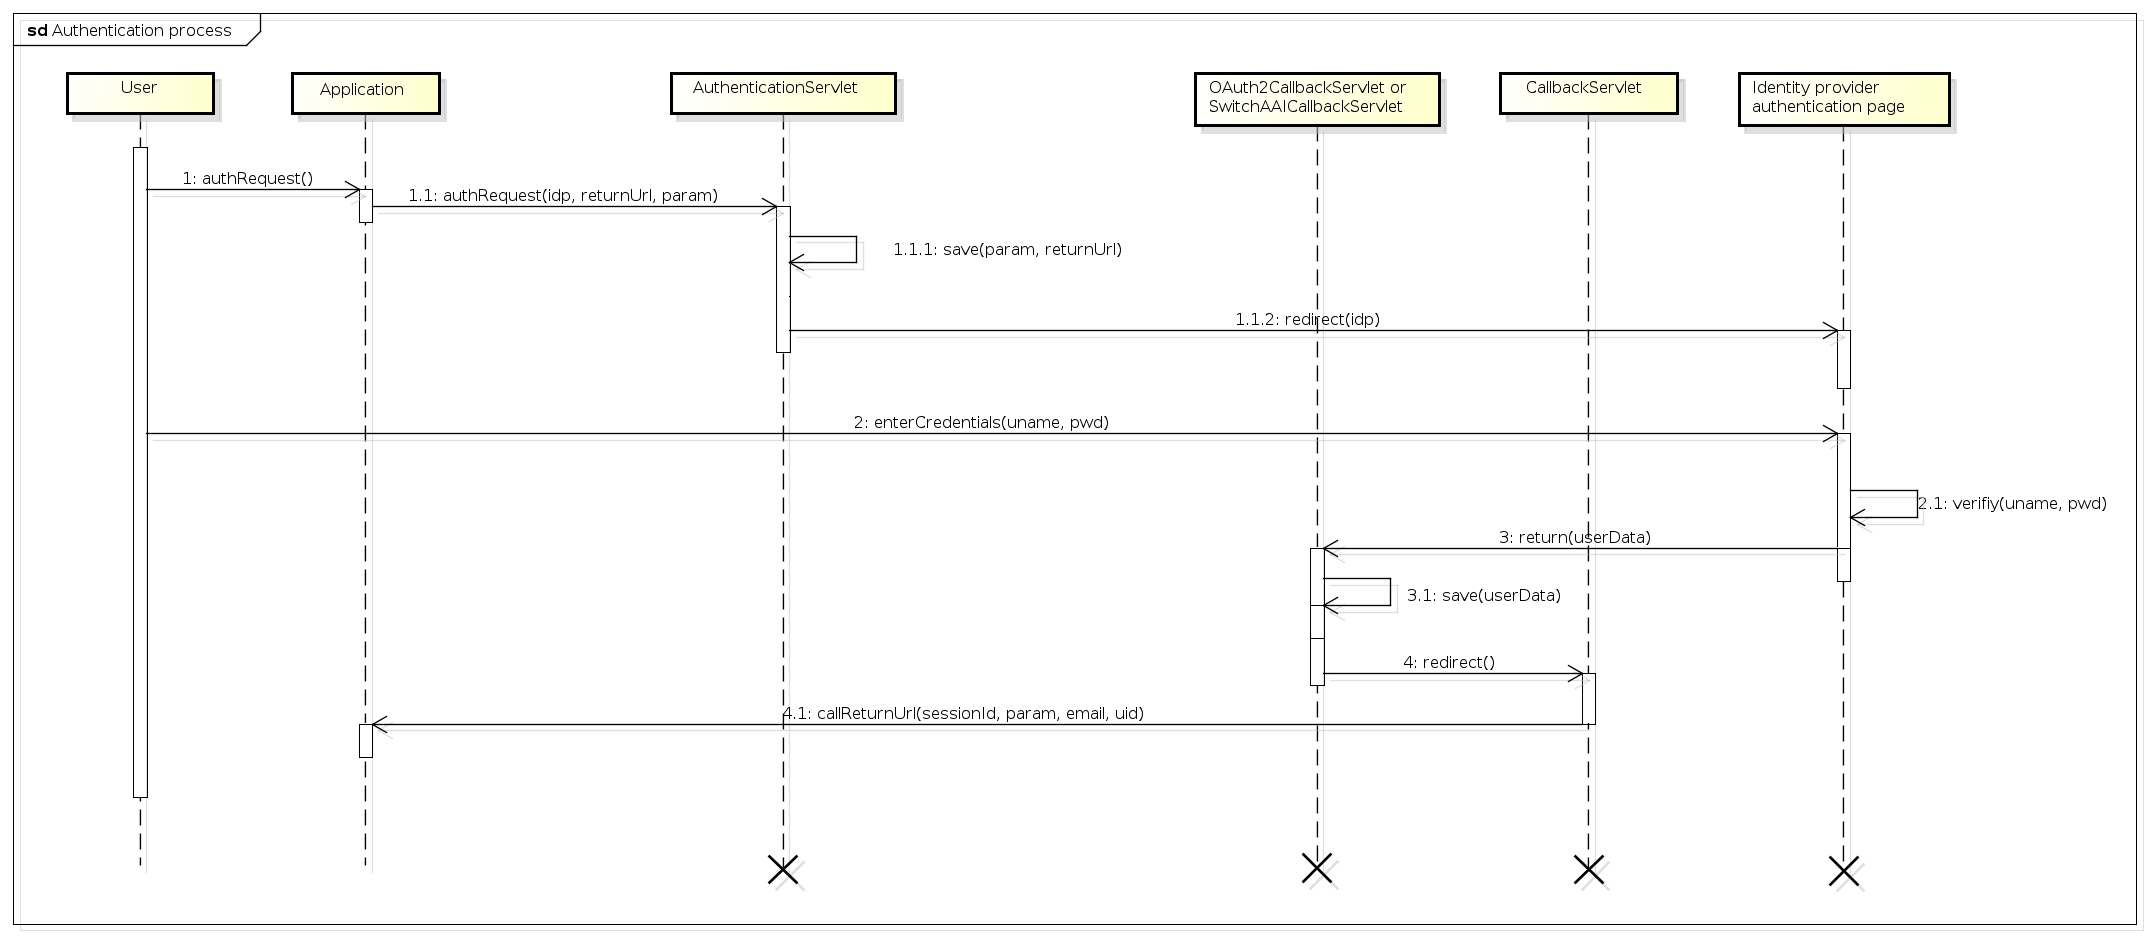
\includegraphics[width=1.0\textwidth]{figs/authentication_process}}
\caption{Authentication process}
\label{fig:auth_process}
\end{figure}

%\paragraph*{Google authentication} Google uses protocol OAuth to manage the authentication. Because of this different technology, the process of authentication with Google is slightly different from the one with SwitchAAI. \Cref{fig:auth_process_google} shows how it works. The first steps are identical until the identity provider is chosen (for this case Google). The \textit{ParametersServlet} redirects the user to Google where the authentication process takes place. The response from Google is sent back to the \textit{OAuth2CallbackServlet} which verifies the response from Google and reads the user personal information received. If everything was correct, the user is redirected to the page where the certificate can be requested (\textit{certificate-request.xhtml}).
%\begin{figure}[ht]
%\centerline{
%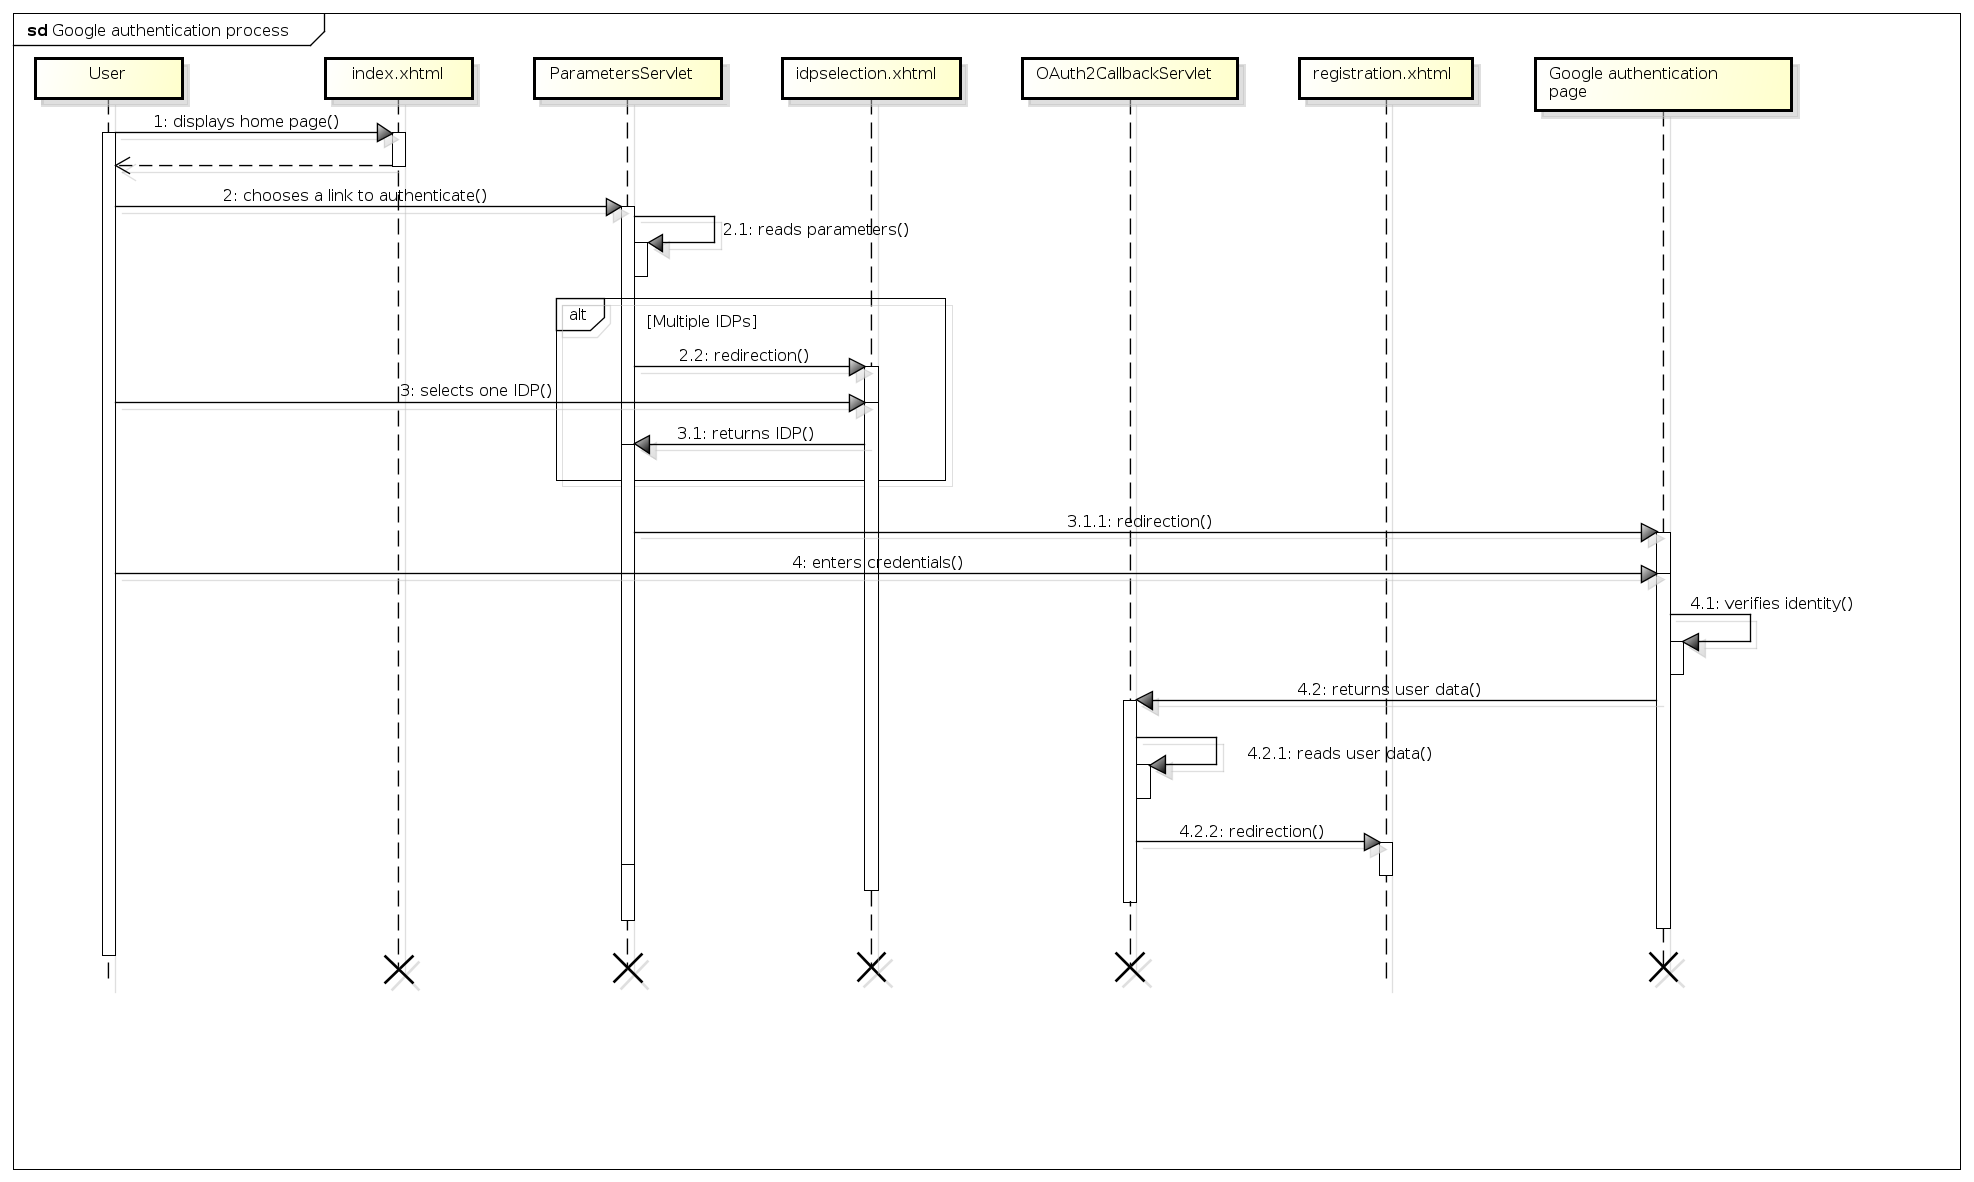
\includegraphics[width=1.0\textwidth]{figs/authentication_process_google}}
%\caption{Authentication process with Google OAuth}
%\label{fig:auth_process_google}
%\end{figure}

\section{Parameters Request}\label{sec:param_request}

Once the user authenticated, the application can propose them to generate the key pair and indicate some parameters that must appear in the certificate. Since, most of the time however, these parameters are the same for a lot of users, \unicert\ allows to predefine parameter sets containing these parameters, so that the user must not define them themselves.

These parameters can be retrieved form the \textit{ParametersServlet}. Therefore, the application must provide the session id received at then end of the authentication process, since these parameters are stored in the user session. The application can then fill the user interface with these parameters in order to simplify the certificate request for the user. More details about these parameters sets can be found in \Cref{sec:simplification_ui}.

\section{Certificate Issuance Process} \label{sec:issuance_process}

The rest of the process is issuance of the certificate. This works in the same way independently of the identity provider used. The process is shown in \Cref{fig:request_process}. This whole process takes place on the page \textit{certificate-request.xhtml}. On this page, the user has to provide following information for the certificate they request: 
\begin{itemize}
\item type of cryptographic values (currently supported: RSA and discrete logarithm)
\item cryptographic parameters: size of key for RSA, values $p,q,g$ for discrete logarithm
\item a private key (generated locally with RSA)
\item a password to encrypt the private key
\item application identifier of the application which the certificate is issued for
\item role in the application the certificate is issued for
\item the identity function that must be applied on the identity information
\end{itemize}

The private key is generated on client side in javascript. The public key corresponding to the generated private key is computed together with a signature (or a proof in case of discrete logarithm setup) to prove the knowledge of the private key. Through javascript, the data listed above (except the private key and the password) are sent to the \textit{CertificateRequestServlet}. In this servlet, the user personal information (also called \textit{user data}) that were received during the authentication process (see \Cref{sec:auth_process}) are used in combination with the identity function to generate the \textit{identity data} that will be included in the certificate. All the processes described until here are realized by the \textit{unicert-authentication} component. The data received and the identity data are then transmitted to the \textit{unicert-issuer} component. This second component verifies the data received and issues the certificate as requested, publishes it on \uniboard and returns it to the \textit{unicert-authentication} component which returns it to the user. In parallel, the secret key is encrypted with the password and sent by mail to the user through the \textit{unicert-authentication} component.

\begin{figure}[ht]
\centerline{
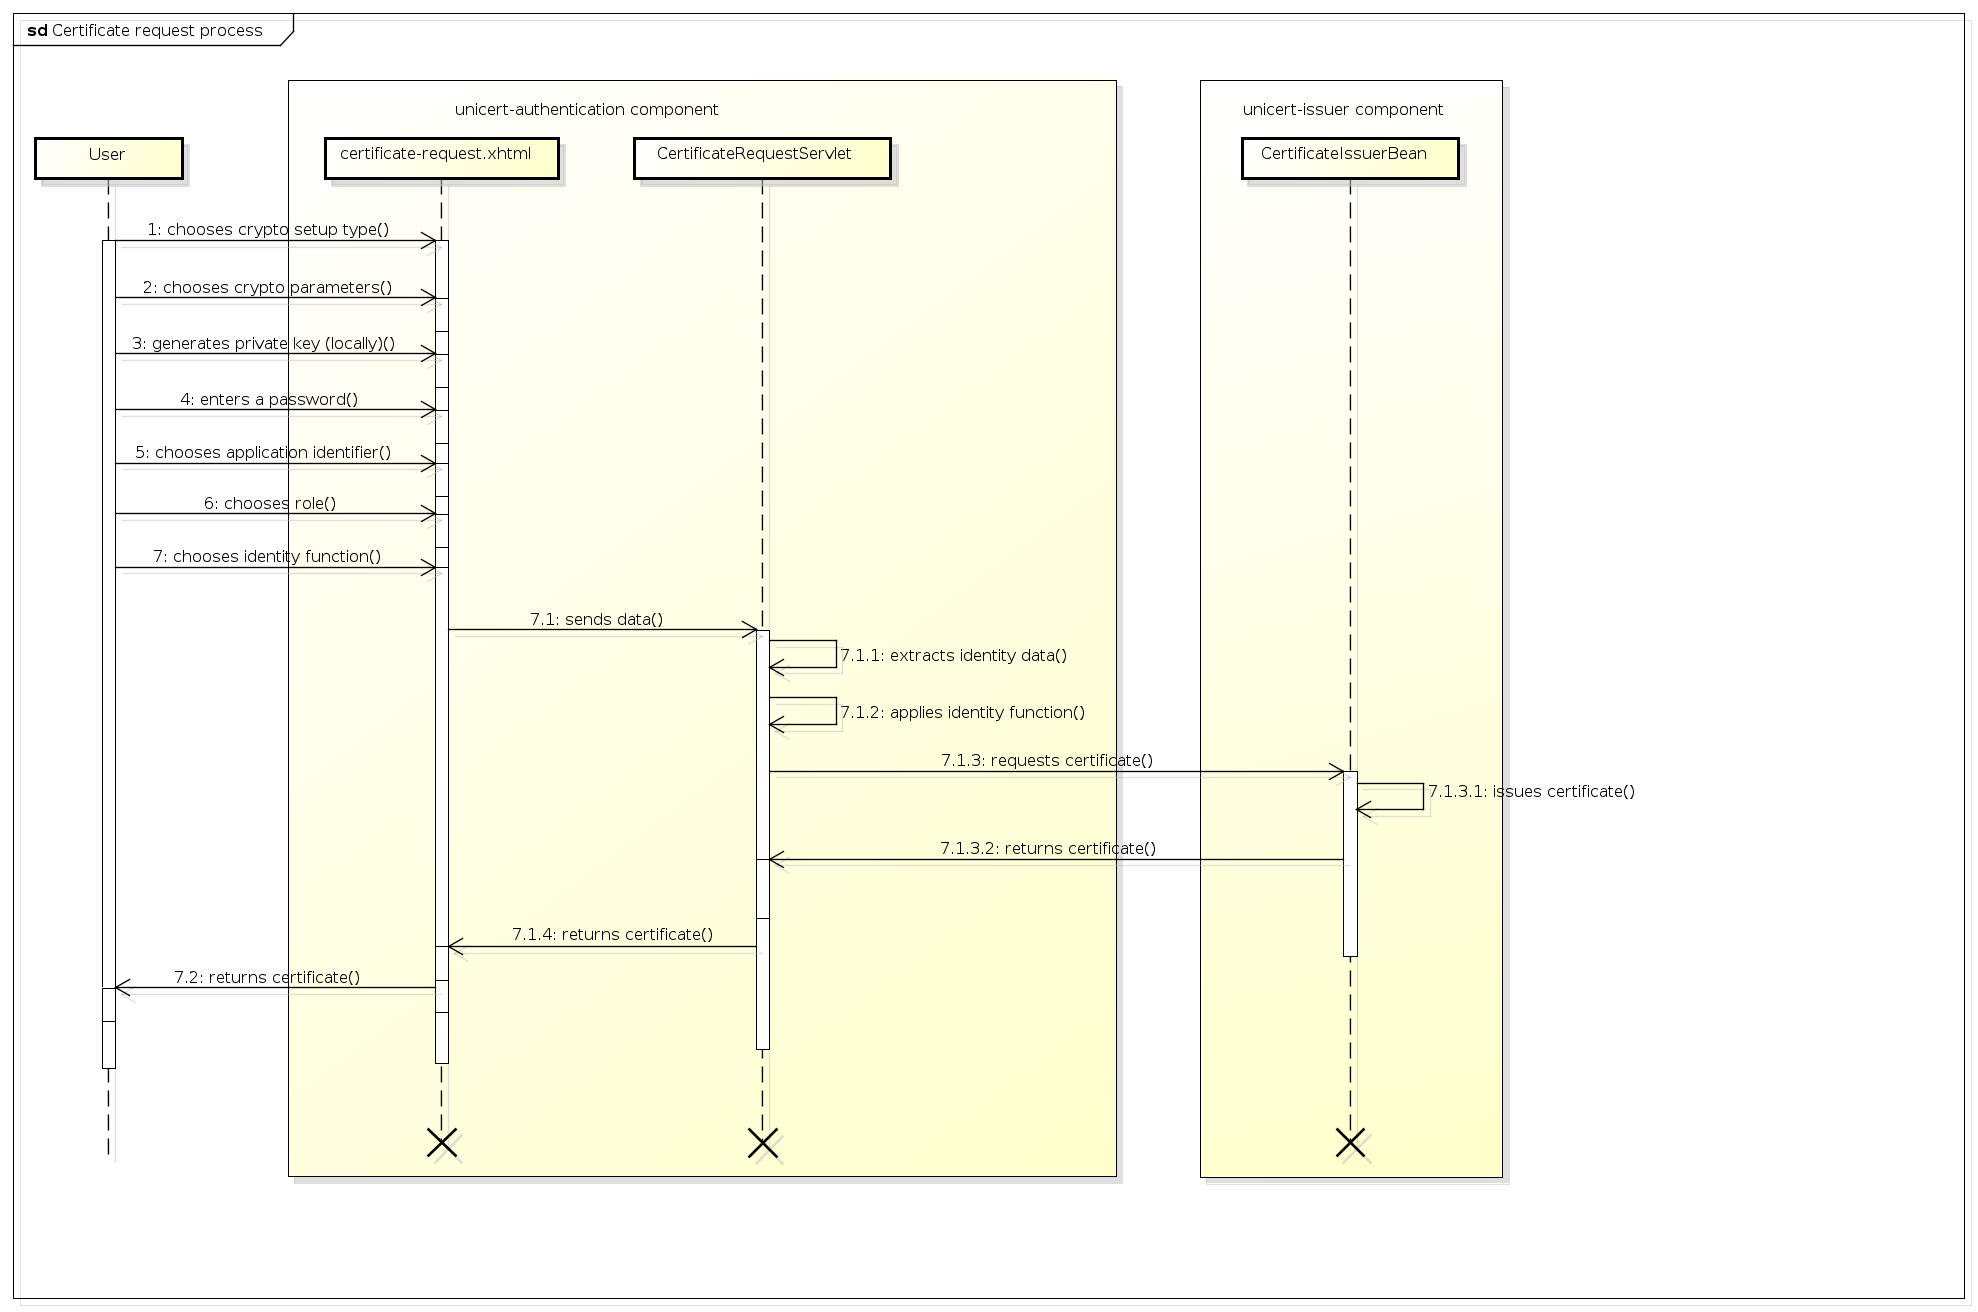
\includegraphics[width=1.0\textwidth]{figs/certificate_request_process}}
\caption{Process of requesting a certificate}
\label{fig:request_process}
\end{figure}

\chapter{Architecture} \label{chap:architecture}
This chapter describes in more details some classes and other architecture concepts of the \textit{unicert-authentication} component and of the \textit{unicert-issuer} component.

\section{unicert-authentication}

\textit{unicert-authentication} is a web application composed of two part, the frontend in JSF/XHTML/Javascript and the backend in Java. The interface between these two parts works over servlets and beans, namely \textit{ParametersServlet}, \textit{CertificateRequestServlet} and \textit{SwitchUserDataBean}. Some important concepts related to the interface between the Java backend and the web frontend as well as some other classes will be described in this section.

\subsection{UserData and IdentityFunction}

The format of the user data returned by the identity provider is not the same for all identity providers. The way these data are transmitted to \unicert\ is also different for various identity providers. These facts require a flexible solution to provide support of multiple identity providers and to allow to easily add a new identity provider.

As already mentioned in \Cref{sec:auth_process}, SwitchAAI use a Shibboleth Apache module for the authentication. This technology requires a user to be logged in before displaying a web page. In this concrete case, it is the page \textit{switchaai.xhtml}. If the user is not logged in, a redirection takes place to SwitchAAI login page. After a successful login, the page \textit{switchaai.xhtml} is displayed to the user, and in the background, a bean called \textit{UserDataBean} is invoked to read the user data returned by Switch in the session. These user data are then stored in an object of the class \textit{SwitchAAIUserData}.

For Google, the user data are returned to a servlet called \textit{OAuth2CallbackServlet} after successful login. This servlet stores the user data in a object of the class \textit{GoogleUserData} and creates the \textit{UserDataBean}. Both \textit{SwitchAAIUserData} and \textit{GoogleUserData} inherits from the \textit{UserData} interface but their content is not the same as shown in \Cref{fig:userdata}, .

\begin{figure}[ht]
\centerline{
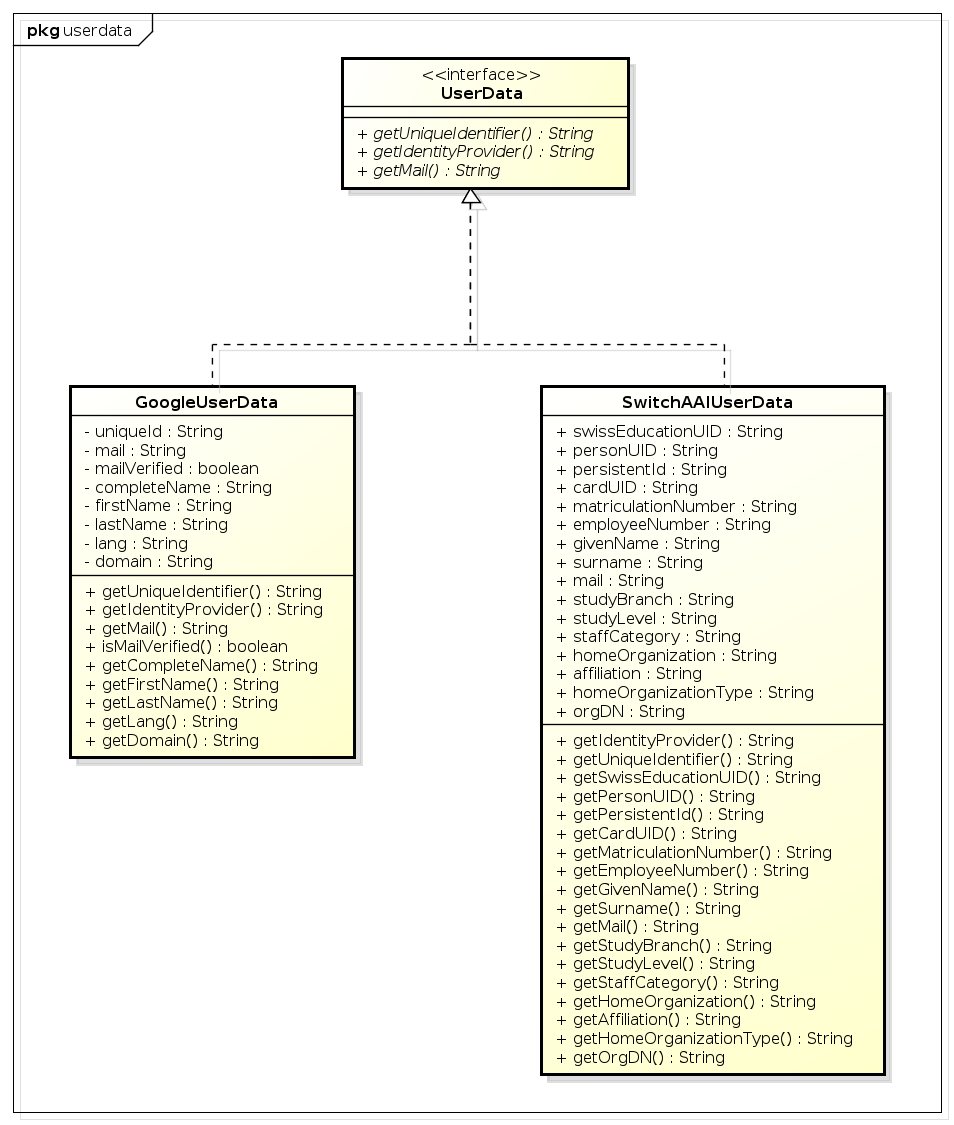
\includegraphics[width=0.6\textwidth]{figs/userdata_class_diagram.png}}
\caption{Class diagram of user data classes}
\label{fig:userdata}
\end{figure}

The \textit{certificate-issuer} component however must know the content of the UserData object in order to be able to extract the data needed in the certificate. Therefore, an identity function is used. There is at least one identity function per identity provider that knows the format of the corresponding user data. So, the GoogleIdentityFunction class knows the fields present in a GoogleUserData object, and the SwitchAAIIdentityFunction knows the content of the SwitchAAIUserData. A concrete IdentityFunction object allows to transform a concrete UserData object into a generic class called \textit{IdentityData} containing the identity information needed for the certificate. This IdentityData object can then be used by the \textit{certificate-issuer} component.

The way how the identity information are extracted from a concrete UserData object is defined in a concrete IdentityFunction object. This process must be adaptable: for example an application could require the e-mail address to appear in certificate, another application could require an other unique identifier, or a third application could require an anonymized form of the e-mail address, and so on. Therefore, multiple IdentityFunction can exist for the same identity provider. In this implementation, there is a standard and an anonymized identity function for each identity provider (\textit{StandardSwitchAAIIdentityFunction}, \textit{StandardGoogleIdentityFunction}, \textit{AnonymizedSwitchAAIIdentityFunction}, \textit{AnonymizedGoogleIdentityFunction}). For SwitchAAI, there is a third variant specially designed for the university of Zürich which uses the student identification number as common name (\textit{ZurichSwitchAAIIdentityFunction}).

The organisation of these classes is shown in \Cref{fig:identity_function_class_diagram}. The \textit{apply} method is the publicly available method extracting the information out of the given UserData object and returning the generated IdentityData object shown in \Cref{fig:identity_data}. Different protected methods are used for this process. \textit{selectCommonName} is responsible for extracting the common name from the UserData. In standard functions, the e-mail address is used. In anonymized function, a hash of the e-mail address is used. In the special function for Zürich, the student identification number is used. \textit{selectUniqueId} is responsible for extracting a unique identifier from the UserData. \textit{putInOtherValues} allows to add information in extensions of the certificate in case it cannot be included in the fields proposed in the IdentityData class. Finally, method \textit{createIdentityData} indicate which fields are put in the IdentityData object. This architecture allows to create subclasses which can overwrite some behaviour of the super class. For example, method \textit{createIdentityData} in anonymized function does not include ''firstname'' and ''surname'' in the IdentityData object as this is done in standard functions.

\begin{figure}[ht]
\centerline{
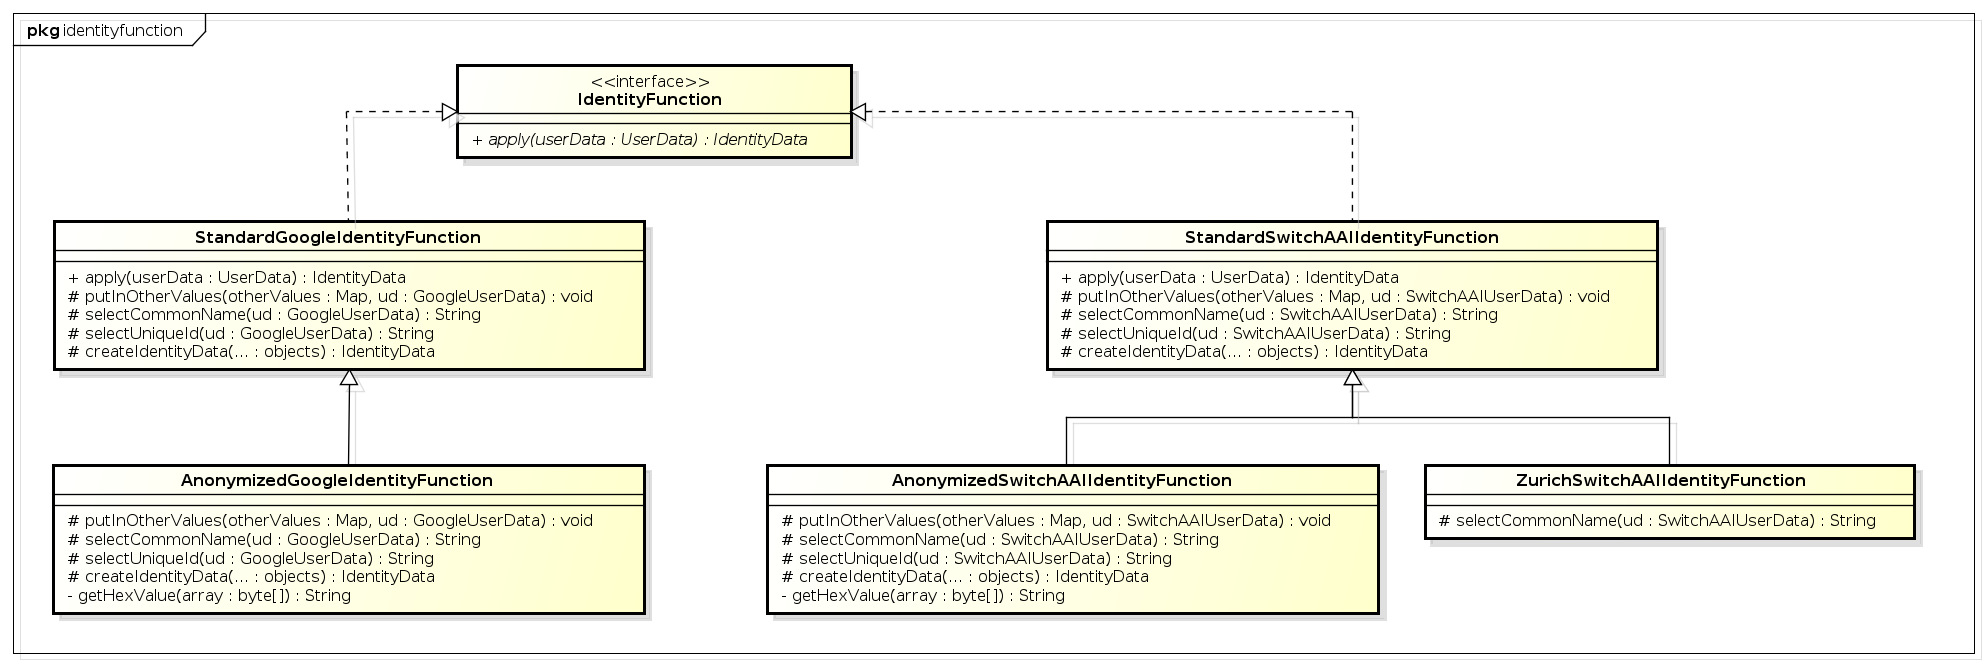
\includegraphics[width=\textwidth]{figs/identity_function_class_diagram.png}}
\caption{Class diagram of the identity function classes}
\label{fig:identity_function_class_diagram}
\end{figure}

\begin{figure}[ht]
\centerline{
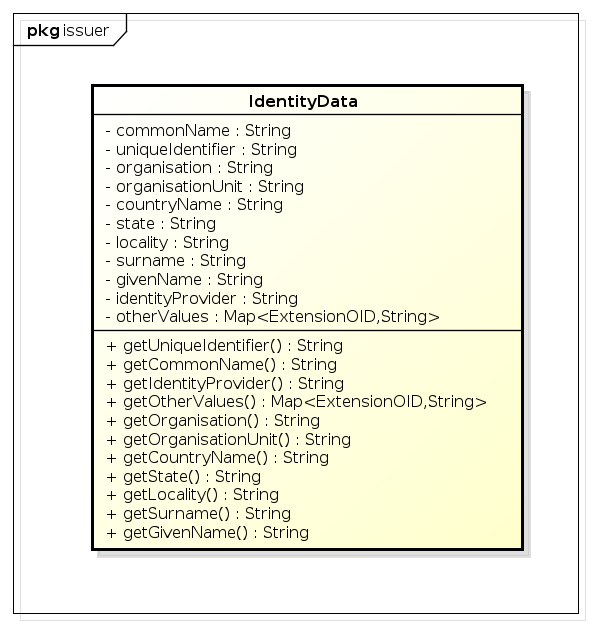
\includegraphics[width=0.4\textwidth]{figs/IdentityData_class.png}}
\caption{IdentityData class}
\label{fig:identity_data}
\end{figure}

\subsection{Error description}

Errors occurring during the issuance process should be communicated in an understandable way to the user. Exception caught in JSF result in a web page displaying the stack trace. This is not intuitive. An exception thrown in the backend result in an HTTP 500 JSON response with an error code and a default error description. Since the issuance request is done over Ajax, the response is also received through Ajax. The error code is then read in Javascript and the corresponding error description is selected in the language file. This message is then displayed to the user.

\subsection{Javascript cryptography}

In the frontend, some cryptographic computation must be realized in Javascript. It concerns the generation of the key pair and the computation of the signature and proofs sent to the backend. In Javascript, a BigInteger library called Leemon \cite{leemon} is used to represent big integers. The needed cryptographic primitives are implemented on top. Because of the bad performance of Javascript in some browsers, some of these primitives have been implemented in an asynchronous way in order to avoid Javascript time outs.

These signatures/proofs generated are verified in the backend using a library called UniCrypt. So, the generation of the signatures and proofs in Javascript must be completely compatible with UniCrypt. Therefore, hash function SHA-256 is used on both side. Recursive hash method is used on UniCrypt side and the equivalent is generated on Javascript side. Strings are considered encoded in UTF-8 and big integers as big endian. 

\section{unicert-issuer}

\textit{unicert-issuer} is an EJB component responsible for the issuance of the certificate. The main class is the \textit{CertificateIssuer} EJB which checks the data received and issues the certificate. Some other classes used in this process will be described in this section.

\subsection{CryptographicSetup}

The class \textit{CryptographicSetup} is a container for all cryptographic values that are submitted by the user and that must be included in the certificate or verified in the \textit{unicert-issuer} component. Two concrete CryptographicSetup exist: \textit{DiscreteLogSetup} and \textit{RSASetup} as shown in \Cref{fig:cryptographic_setup_class_diagram}. They both include all values that define such a setup and the signature or proof generated in the frontend. Objects of these classes are created by the \textit{unicert-authentication} component on certificate request.

\begin{figure}[ht]
\centerline{
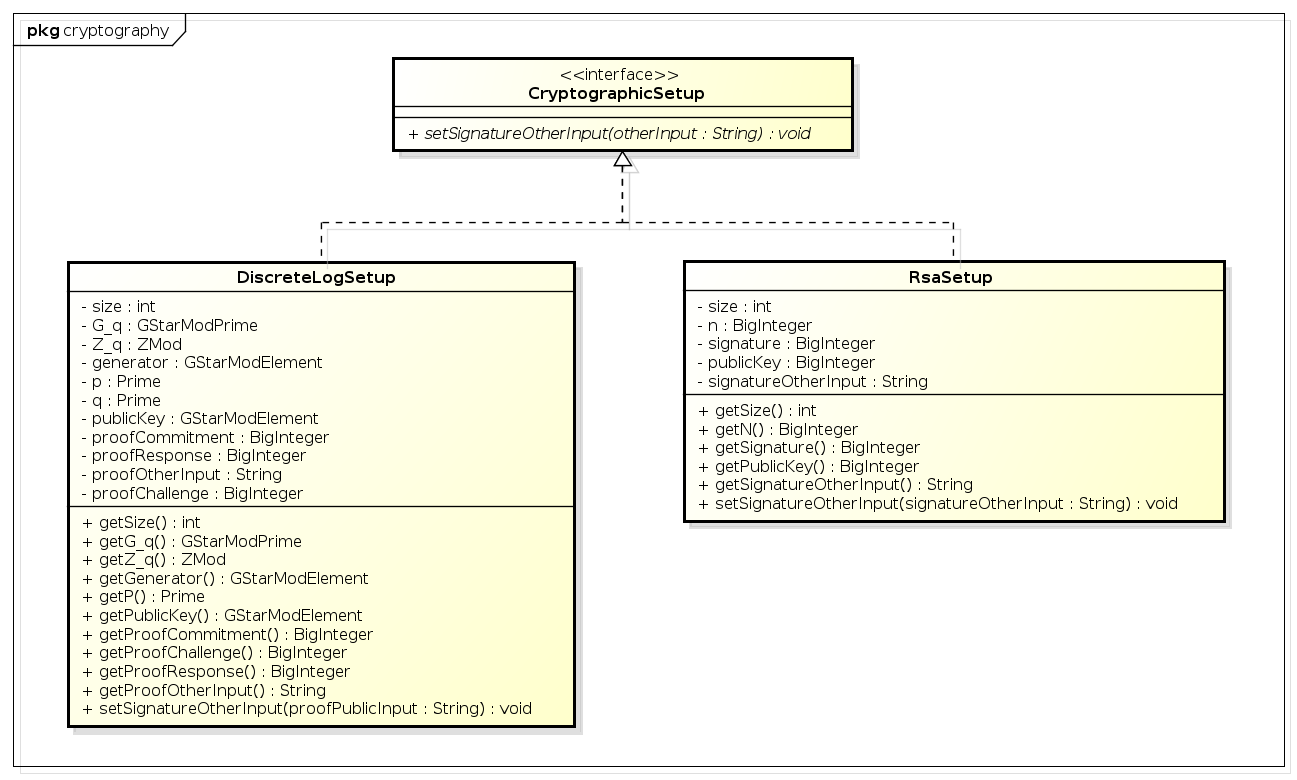
\includegraphics[width=\textwidth]{figs/cryptographic_setup_class_diagram.png}}
\caption{Class diagram of the cryptographic setup classes}
\label{fig:cryptographic_setup_class_diagram}
\end{figure}

\subsection{Certificate class}

Certificate class is the Java representation of the X.509 certificate that is issued. The fields that appear in that certificate are stored here together with the PEM format of the issued certificate as shown in \Cref{fig:certificate}. When posting the certificate on \uniboard, a JSON representation of this class is created through the method \textit{toJSON}. This allows \uniboard\ to make query on the content of a certificate. The listing below shows the schema of the generated JSON certificate.

\begin{figure}[ht]
\centerline{
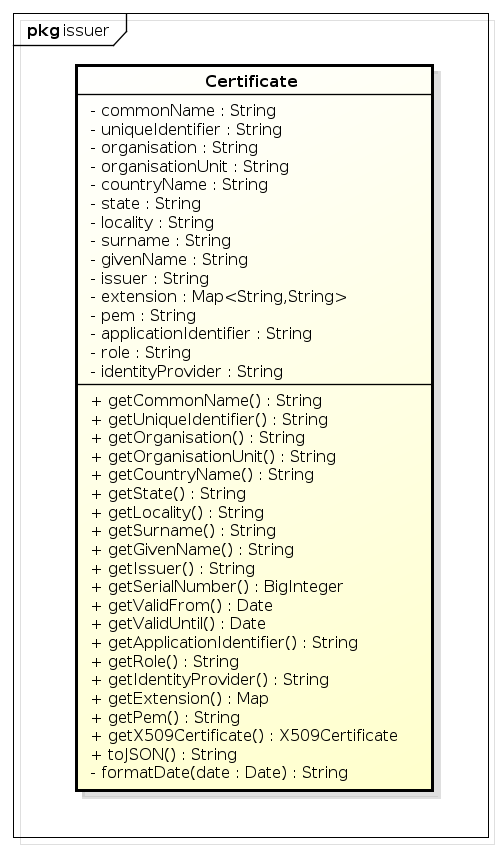
\includegraphics[width=0.4\textwidth]{figs/certificate_class.png}}
\caption{Certificate class}
\label{fig:certificate}
\end{figure}

\begin{lstlisting}[language=json,firstnumber=1]
{
	"title": "Schema for UniCert certificates",
	"description": "This schema describes the format of a UniCert certificate in JSON format",
	"type":"object",
	"$schema": "http://json-schema.org/draft-04/schema",
	"properties": {
		"commonName": {
			"type": "string",
			"description": "Common name of certificate owner"
		},	
		"uniqueIdentifier": {
			"type": "string",
			"description":  "Unique identifier of certificate owner"
		},
		"organisation": {
			"type": "string",
			"description": "Organisation of certificate owner"
		},
		"organisationUnit": {
			"type": "string",
			"description": "Organisation unit of certificate owner"
		},
		"countryName": {
			"type": "string",
			"description": "Country of certificate owner"
		},
		"state": {
			"type": "string",
			"description": "State of certificate owner"
		},
		"locality": {
			"type": "string",
			"description": "Locality certificate owner"
		},
		"surname": {
			"type": "string",
			"description": "Surname of certificate owner"
		},
		"givenName": {
			"type": "string",
			"description": "Given name of certificate owner"
		},
	   	"issuer": {
			"type": "string",
			"description": "Issuer of the certificate"
		},
		"serialNumber": {
			"type":"string",
			"description": "Serial number of the certificate"
		},
		"validFrom": {
			"type": "string",
			"description": "Date when certificate starts to be valid"
		},
		"validUntil": {
			"type": "string",
			"description": "Date when certificate stops to be valid"
		}, 
		"applicationIdentifier": {
			"type": "string",
			"description": "Application the certificate has been issued for"
		},
		"role": {
			"type":"array",
			"description": "Role inside an application the certificate has been issued for",
			"items": {
				"type":"string"
			}
		},
		"identityProvider": {
			"type": "string",
			"description": "Identity provider used to verify the identity of the certificate owner"
		},
		"pem": {
			"type": "string",
			"description": "Certificate in PEM format"
		}
	},
	"required": ["commonName", "issuer", "serialNumber", "validFrom", "validUntil", "identityProvider", "pem" ]
}
	
\end{lstlisting}



\chapter{UniCert Particularities} \label{chap:specialities}
This chapter describes in more details some particularities of \unicert.

\section{X.509 Certificate Extensions}

Some special information must be added by \unicert\ in the issued certificate, like the identity provider used for the authentication, the application and the role the certificate is issued for. This information cannot really be included in existing X.509 fields. So, we defined some extensions for each of these elements. In X.509 certificates, an extension must always be identified by an object identifier (OID). The Bern University of Applied Sciences own a group OID: 1.3.6.1.4.1.13305. Following subgroup is reserved for \unicert\: 1.3.6.1.4.1.13305.1.101.x. \Cref{t:oids} presents the elements included in the certificate and their corresponding OIDs. The content of these extensions are always ASN1 strings.


\begin{table}[ht]

\centering
\begin{tabular}{|c|c|}
  \hline
  Element & OID\\
  \hline
  Identity provider & 1.3.6.1.4.1.13305.1.101.1 \\
  Application identifier & 1.3.6.1.4.1.13305.1.101.2 \\
  Role & 1.3.6.1.4.1.13305.1.101.3 \\
  Language (only for Google) & 1.3.6.1.4.1.13305.1.101.4 \\
  Test extension & 1.3.6.1.4.1.13305.1.101.999 \\
  \hline
\end{tabular}
\caption{OIDs}
\label{t:oids}
\end{table}

\section{JNDI Propreties for \textit{unicert-issuer}}

To work properly, \textit{unicert-issuer} require some configuration values. These values are defined as JNDI properties. \Cref{t:jndi1} shows what are these values. They are stored in a property set called \textit{unicertProps}.

\begin{table}[ht]

\centering
\begin{tabular}{|l|l|}
  \hline
  Property & Description\\
  \hline
  keystoreExternal & If the keystore must be loaded from an external location\\
  keystorePath & Path to the keystore containing the certificate and private key\\ &  of \unicert\ for signing issued certificates\\
  keystorePass & Password for the keystore \\
  privateKeyPass & Password used to protect private key of \unicert\ certificate \\
  issuerId & Name of the issuer of the generated certificates \\
  validityYears & Time slot in which the certificate is valid (2 years) \\
  uniboardURL & URL of \uniboard\ webservice (if not indicated, certificates are\\ & not published)\\
  googleRedirectURI & URL of the callback servlet after Google OAuth2 authentication \\
  googleClientID & OAuth2 credentials for Google authentication\\
  googleClientSecret & OAuth2 credentials for Google authentication\\
  \hline
\end{tabular}
\caption{JNDI properties for \textit{unicert-issuer}}
\label{t:jndi1}
\end{table}

\section{Simplification of the User Interface}\label{sec:simplification_ui}

As described in \Cref{sec:issuance_process}, when the user requests a certificate, they have to provide, among other, following information:

\begin{itemize}
\item type of cryptographic values (currently supported: RSA and discrete logarithm)
\item cryptographic parameters: size of key for RSA, values $p,q,g$ for discrete logarithm
\item application identifier of the application the certificate is issued for
\item role in the application the certificate is issued for
\item the identity function that must be applied on the user's personal information
\end{itemize}

Most of the time however, these values are the same for a lot of users. For example, when a voter wants to issue a voter certificate for \univote, the cryptographic values, the application identifier (in this case \univote) and the role (in this case \textit{Voter}) are the same for all users that request a certificate. Even the identity function is the same for all voters inside a given election. So, it is unintuitive to ask each user to enter all these data. Therefore, a feature has been implemented allowing to preset all these values. It works with JNDI properties. The administrator can define multiple JNDI property sets giving them a name like ''/unicert/mypropertyset''. In this property set, the administrator can define the properties they want not to be filled by the user. The ones that are not defined must then be filled by the user in the certificate request process. The property set is loaded by the \textit{ParametersServlet} which receives the name of the property set to load through the link on which the user has clicked to start the authentication process, for example ''authenticate?params=mypropertyset''. If no property set is indicated, a default property set is loaded containing only the identity providers supported. All others information must be filled by the user. \Cref{t:jndi2} shows the JNDI properties that can be preset in a property set.

\begin{table}[ht]

\centering
\begin{tabular}{|l|l|l|l|}
  \hline
  Property & Description & Possible values & \\
  \hline
  identityProvider & The identity provider to & ''SwitchAAI'', & Mandatory\\ & use for authentication & ''Google'', & \\ & & ''SwitchAAI,Google'' & \\
  keyType & Cryptographic setup type & ''RSA'', ''DiscreteLog'' & Optional\\
  keySize & Size of RSA keys & integer & Optional\\
  primeP & Value of prime p & base 10 representation & Optional\\
  primeQ & Value of prime q & base 10 representation & Optional\\
  generator & Value of generator & base 10 representation & Optional\\
  applicationIdentifier & Application identifier & string & Optional\\
  role & Role & string & Optional\\
  identityFunctionIndex & Index of identiy function & integer & Optional\\
  & to select in dropdown & & \\
  \hline
\end{tabular}
\caption{JNDI properties for presets in user interface}
\label{t:jndi2}
\end{table}



%%%%%%%%%%%%%%%%%%%%%%%%%%%%%%%%%%%%%%%%%%%%%%%%%%%%%%%%%%%%%%%%%%%%%%%%
\bibliographystyle{plain} \bibliography{arch-spec}
%%%%%%%%%%%%%%%%%%%%%%%%%%%%%%%%%%%%%%%%%%%%%%%%%%%%%%%%%%%%%%%%%%%%%%%%

\end{document}
